\documentclass[a4paper, 12pt]{article}
\usepackage[T2A]{fontenc}
\usepackage[utf8]{inputenc}
\usepackage[english,russian]{babel}
\usepackage{amsmath, amsfonts, amssymb, amsthm, mathtools, misccorr, indentfirst, multirow, multicol}
\usepackage{wrapfig}
\usepackage{graphicx}
\usepackage{subfig}
\usepackage{adjustbox}
\usepackage{pgfplots}

\usepackage{geometry}
\geometry{top=20mm}
\geometry{bottom=20mm}
\geometry{left=20mm}
\geometry{right=20mm}
\newcommand{\angstrom}{\textup{\AA}}

\title{Лабораторная работа № 4.3.6\\Саморепродукция}
\author{Нехаев Александр. гр. 654}

\begin{document}
\maketitle
\newpage
\tableofcontents
\newpage
\section{Введение}
\paragraph{Цель работы} Изучение явления саморепродукции и применение его к измерению параметров периодических структур.
\paragraph{В работе используются} лазер, кассета с сетками, мира, короткофокусная линза с микрометрическим винтом, экран, линейка.
\paragraph{Теоретическое введение}
Выражение для плоской монохроматической волны имеет вид 
	\begin{equation}\label{eq:wave}
		E(\mathbf{r}, t) = a_0e^{-i(\omega t - \mathbf{kr} - \psi_0)}, 
	\end{equation}
	где $a_0$ - амплитуда, $\omega$ - круговая частота, $\mathbf{k} = (u, v, q)$ - волновой вектор , $\psi_0$ - начальная фаза. Колебания происходят синфазно во всех точках плоскости:
	\begin{equation}\label{eq:kr}
		\mathbf{kr} = ux + vy + \sqrt{k^2 - u^2 - v^2}\cdot z = const.
	\end{equation}
	
	Для плоской волны \eqref{eq:wave} комплексную амплитуду можно представить в виде
	\begin{equation}\label{eq:to_z}
		f(x, y, z) = a_oe^{i\psi_0}e^{ux+vy}e^{\sqrt{k^2 - u^2 - v^2}\cdot z} = f(x, y, 0)e^{\sqrt{k^2 - u^2 - v^2}\cdot z}.
	\end{equation}
	
	Пусть плоская волна падает нормально на транспарант, расположенный в плоскости $z = 0$. Комплексную амплитуду волны в плоскости $z = 0_+$ получаем, умножив комплексную амплитуду на входе в транспарант на функцию пропускания транспаранта $t(x, y)$. Для простоты далее будем рассматривать случай $t(x, y) = t(x)$. Если функция пропускания периодична с пространственным периодом $d$, то комплексная амплитуда на выходе также будет периодической функцией с периодом $d$
	\begin{equation}\label{eq:decomp}
		f(x, 0_+) = \sum\limits_{-\infty}^{+\infty} c_ne^{iu_nx} = \sum\limits_{-\infty}^{+\infty} c_ne^{i\frac{2\pi}{d}nx},
	\end{equation}
	где коэффициенты $c_n$ можно найти с помощью формулы
	\begin{equation}\label{eq:coeff}
		c_n = \frac{1}{d} \int\limits_{-d/2}^{d/2} f(x, 0_+)e^{-i\frac{2\pi}{d}nx}
	\end{equation}
	
	Для нахождения комплексной амплитуды волны в произвольной плоскости $z = const$ нужно домножить комплексные амплитуды плоских волн в суперпозиции \eqref{eq:decomp} на соответствующий фазовый множитель (равенство \eqref{eq:kr}):
	\begin{equation}\label{eq:to_zz}
		f(x, z) = \sum\limits_{-\infty}^{+\infty} c_ne^{iu_nx}e^{\sqrt{k^2 - u_n^2}\cdot z}
	\end{equation}
	То есть, каждая плоская волна приобретает дополнительный набег фаз $\varphi_n$. Для параксиальных волн $(u_n \ll 1)$
	\begin{equation}\label{eq:parax}
		\varphi_n = \sqrt{k^2 - u_n^2}\cdot z \approx kz - \frac{u_n^2}{2k}z
	\end{equation}
	Таким образом, для любых двух плоских волн разность набегов фазы равна
	\begin{equation}\label{eq:phase}
		\Delta\varphi_{n, m} = (u_m^2 - u_n^2)\frac{z}{2k} = (m^2 - n^2)\frac{\pi\lambda}{d^2}z.
	\end{equation}
	
	В плоскости
	\begin{equation}
		z_N = \frac{2d^2}{\lambda}N
		\label{eq:8}
	\end{equation}
	разница набегов фаз становится кратной $2\pi$. Поэтому в результате интерференции волн в этой плоскости получается изображение, тождественное исходному периодическому объекту. Это и есть \textit{эффект саморепродукции}.
	\section{Схема установки}
	\begin{figure}[h]
		\centering
		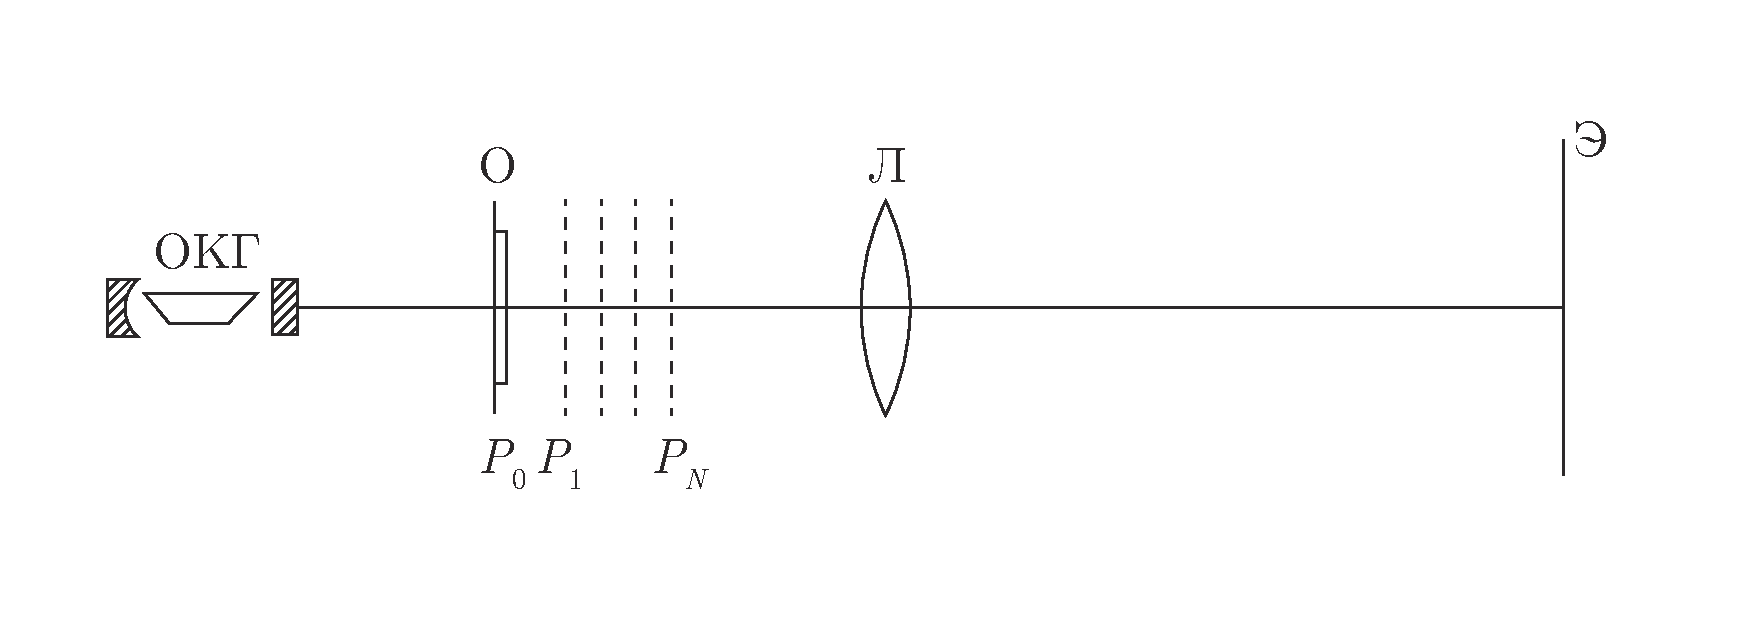
\includegraphics[scale=0.6]{scheme.pdf}
		\caption{Схема экспериментальной установки}
	\end{figure}
	\section{Ход работы}
	В нашем эксперименте $\lambda = 532\,\text{нм}$.
	\subsection{Исследование двумерных решеток}
	\subsubsection{Определение периода решеток по их пространственному спектру}
	\begin{enumerate}
		\item Закрепим кассету с двумерными решетками (сетками) вблизи выходного окна лазера так, чтобы в окошке под отверстием с сеткой был виден её номер.
		\item Для каждой сетки определим расстояние $x$ между соседними дифракционными максимумами на экране: измерим расстояние $X$ между двумя достаточна удалёнными друг от друга максимумами и поделим на число промежутков $m$ между ними ($x=X/m=f\left(\text{№}\right)$). По формуле $d=\frac{L\lambda}{x}$, определим период решетки $d$. Результаты занесем в таблицу \ref{tab:1}.
		\begin{table}[h]
			\centering
			\begin{tabular}{|c|c|c|c|c|c|}
				\hline
				№ & 1 & 2 &  3 & 4 & 5\\
				\hline
				$X$, см & 7 & 4.8 & 4.8 & 2.5 & 1.4\\
				$m$ & 2 & 2 & 4 & 4 & 3\\
				$x$, мм & 35 & 24 & 12 & 6.25 & 4.67\\
				$d$, мкм & 20.52 & 29.925 & 59.85 & 114.912 & 153.9\\
				\hline
			\end{tabular}
			\caption{Исследование с помощью спектра. $L=135$ см.}
			\label{tab:1}
		\end{table}
	\end{enumerate}
	\subsubsection{Определение периода решёток по изображению, увеличенному с помощью линзы}
	\begin{enumerate}
		\item Закрепим короткофокусную линзу на небольшом расстоянии от лазера. Временно удалим кассету с сетками из луча и центрировкой линзы совместим световое пятно, сформированное линзой, с положением луча на экране в отсутствие линзы. Передвигая линзу с помощью микрометрического винта, сначала убедимся, что световое пятно на экране неподвижно, затем переместим линзу как можно ближе к кассете.
		\item Установим кассету с сетками между лазером и линзой и, перемещая её вдоль оси системы, получим на экране увеличенное изображение одной из сеток.\\
			Изображение сетки периодически повторяется в пространстве, поэтому для того, чтобы среди множества репродуцированных изображений сетки можно было выделить её геометрическое изображение, на одну из сеток наложена тонкая проволочка, т. е. непериодический объект, изображение которого не репродуцируется. Найдем резкое изображение проволочки; убедимся, что при смене сеток резкость изображений не нарушается.
			\item Определим размеры $D$ клеток на экране. Результаты занесем в таблицу \ref{tab:2}
			\begin{table}[h]
				\centering
				\begin{tabular}{|c|c|c|c|c|c|}
					\hline
					№ & 1 & 2 & 3 & 4 & 5\\
					\hline
					$D$, мм & 0.5 & 5.5 & 9 & 3 & 4.5\\
					$m$ & 1 & 7 & 6 & 1 & 1\\
					$d$, мкм & 67.06 & 105.38 & 201.17 & 402.35 & 603.52\\
					\hline
				\end{tabular}
				\caption{Исследование по изображению. $a=16$ см, $b=119.3$ см.}
				\label{tab:2}
			\end{table}
	\end{enumerate}
	\subsubsection{Исследование эффекта саморепродукции с помощью сеток}
	Получим на экране геометрическое изображение сетки. Перемещая линзу с помощью микровинта, определим по нониусной шкале координаты $z_N$ плоскостей саморепродукции, соответствующих чёткому изображению сетки на экране.\par
	Повторим измерения для других сеток.\par
	Для крупных сеток полезно при измерениях строить графики $z_N=f\left(N\right)$, чтобы по формуле (\ref{eq:8}) рассчитаем период сеток $d_\text{реп}=f\left(\text{№}\right)$.
	 \begin{table}[h]
	 	\centering
	 	\begin{tabular}{|c|c|c|c|c|c|}
	 		\hline
	 		№ & \multicolumn{5}{c|}{5}\\
	 		\hline
	 		N & -2 & -1 & 0 & 1 & 2\\
	 		$z_N$, см & 73.2 & 68.2 & 61.7 & 55.2 & 50\\
	 		\hline
	 	\end{tabular}
	 	\begin{tabular}{|c|c|c|c|c|c|c|c|c|c|c|}
	 		\hline
	 		№ & \multicolumn{10}{c|}{4}\\
	 		\hline
	 		N & -5 & -4 & -3 & -2 & -1 & 0 & 1 & 2 & 3 & 4\\
	 		$z_N$, см & 78.9 & 75.5 & 72 & 68.9 & 65.1 & 61.7 & 57.3 & 53.3 & 50.7 & 47.4\\
	 		\hline
	 	\end{tabular}
	 	
	 	\begin{tabular}{|c|c|c|c|c|c|c|c|c|c|}
	 		\hline
	 		№ & \multicolumn{9}{c|}{3}\\
	 		\hline
	 		N & -4 & -3 & -2 & -1 & 0 & 1 & 2 & 3 & 4\\
	 		$z_N$, см & 78.9 & 75.5 & 72 & 68.9 & 65.1 & 61.7 & 57.3 & 53.3 & 50.7 \\
	 		\hline
	 	\end{tabular}
	 	\caption{Исследование репродукции}
	 \end{table}
	 \begin{figure}[h]
	 	\centering
	 	\begin{minipage}{0.49\textwidth}
	 		\begin{tikzpicture}
	 		\begin{axis}[
	 			title={Сетка №5},
	 			xlabel={$N$},
	 			ylabel={$z_N$, см},
	 			xmin=-2,
	 			xmax=2,
	 			ymin=50,
	 			ymax=75,
	 			ymajorgrids=true,
   				xmajorgrids=true,
	 			grid style=dashed,
	 			width=\textwidth
	 		]
	 		\addplot+[color=black,
				mark=square,
				only marks,
				error bars/.cd,
				y dir=both, y explicit,
				x dir=both, x explicit
			]
			coordinates {
				(-2,73.2)+-(0,0.5)
				(-1,68.2)+-(0,0.5)
				(0,61.7)+-(0,0.5)
				(1,55.2)+-(0,0.5)
				(2,50)+-(0,0.5)
			};
			\addplot[
				domain=-2:2,
				samples=100,
				color=black,
			]
			{-5.94*x+61.66};
	 		\end{axis}
	 		\end{tikzpicture}
	 	\end{minipage}
	 	\hfill
	 	\begin{minipage}{0.49\textwidth}
	 		\begin{tikzpicture}
	 			\begin{axis}[
	 				title={Сетка №4},
	 				xlabel={$N$},
	 				ylabel={$z_N$, см},
	 				xmin=-5,
	 				xmax=4,
	 				ymin=45,
	 				ymax=80,
	 				ymajorgrids=true,
   					xmajorgrids=true,
	 				grid style=dashed,
	 				width=\textwidth
	 			]
	 			\addplot+[
	 				color=black,
					mark=square,
					only marks,
					error bars/.cd,
					y dir=both, y explicit,
					x dir=both, x explicit
	 			]
	 			coordinates{
	 				(-5,78.9)+-(0,0.5)
	 				(-4,75.5)+-(0,0.5)
	 				(-3,72)+-(0,0.5)
	 				(-2,68.9)+-(0,0.5)
	 				(-1,65.2)+-(0,0.5)
	 				(0,61.7)+-(0,0.5)
	 				(1,57.3)+-(0,0.5)
	 				(2,53.3)+-(0,0.5)
	 				(3,50.7)+-(0,0.5)
	 				(4,47.4)+-(0,0.5)
	 			};
	 			\addplot[
	 				domain=-5:4,
	 				samples=100,
	 				color=black
	 			]{-3.57*x+61.296};
	 			\end{axis}
	 		\end{tikzpicture}
	 	\end{minipage}
	 	\\
	 	\begin{minipage}{0.49\textwidth}
	 		\begin{tikzpicture}
	 			\begin{axis}[
	 				title={Cетка №3},
	 				xlabel={$N$},
	 				ylabel={$z_N$, см},
	 				xmin=-4,
	 				xmax=4,
	 				ymin=45,
	 				ymax=75,
	 				ymajorgrids=true,
   					xmajorgrids=true,
	 				grid style=dashed,
	 				width=\textwidth
	 			]
	 			\addplot+[
	 				color=black,
					mark=square,
					only marks,
					error bars/.cd,
					y dir=both, y explicit,
					x dir=both, x explicit
	 			]
	 			coordinates{
	 				(-4,73.9)+-(0,0.5)
	 				(-3,70)+-(0,0.5)
	 				(-2,67.3)+-(0,0.5)
	 				(-1,64.9)+-(0,0.5)
	 				(0,61.7)+-(0,0.5)
	 				(1,59.3)+-(0,0.5)
	 				(2,56.5)+-(0,0.5)
	 				(3,51.9)+-(0,0.5)
	 				(4,49.4)+-(0,0.5)
	 			};
	 			\addplot[
	 				domain=-4:4,
	 				samples=100,
	 				color=black
	 			]{-2.99*x+61.66};
	 			\end{axis}
	 		\end{tikzpicture}
	 	\end{minipage}
	 \end{figure}
	 Рассчитаем значения для $d$ и занесем их в таблицу \ref{table:reproduct_net}.\par
	 \begin{table}[h!]
	 	\centering
	 	\begin{tabular}{|c|c|c|c|}
	 		\hline
	 		№ & 3 & 4 & 5\\
	 		\hline
	 		$d$, мкм & 89.2$\pm$17.8 & 97.4$\pm$19.5 & 125.6$\pm$25.1\\
	 		\hline
	 	\end{tabular}
	 	\caption{Рассчет $d$ через репродукцию.}
	 	\label{table:reproduct_net}
	 \end{table}
	 \subsection{Исследование решеток миры}
	 Ввиду сложности настройки на определенный элемент миры предлагается следующий порядок измерения периодов: для одного элемента сначала по саморепродукции, затем по увеличенному изображению и, наконец, по спектру.
	 \begin{enumerate}
	 	\item Рассмотрим миру в отраженному свете. Убедимся, что самые мелкие решетки расположены внизу. Найдем элемент миры с номером 25.
	 	\item Установим миру на место кассеты (стекло миры обращено к линзе) таким образом, чтобы на экране было видно резкое увеличенное изображение цифры 25. Перемещая рейтер с мирой перепендикулярно лучу, осветим одну из ближайших сеток. Перемещением миры подведем пятно лазера к центру выбранной решетки и уточним настройку на геометрическое изображение с помощью микровинта.
	 	\item Перемещая линзу с помощью микрометрического винта, определим по нониусной шкале координату плоскости, соответствующей изображению миры на экране по законам геометрической оптики, и координаты плоскостей саморепродукции.
	 	\item Вернем линзу в положение, соответствующее изображению по законам геометрической оптики. Определим параметры изображения миры на экране; измерим расстояние от линзы до экрана и до миры.
	 	\item Поворотом линзы в рейтере вокруг вертикальной оси выведем линзу из луча и проведем измерения спектра миры.
	 	\item Потворим всю серию измерений для миры с номером 20.
	 	\item Занесем результаты измерений в таблицу 6.
	 	\begin{table}[h]
	 		\centering
	 		\begin{tabular}{|c|c|c|c|}
			\hline
			\multicolumn{2}{|c|}{По спектру} & \multicolumn{2}{c|}{По изображению} \\ \hline
			Мира 25        & Мира 20         & Мира 25          & Мира 20          \\ \hline
			l = 1.8        & l = 1.35        & p = 0.1          & p = 0.14         \\ \hline
			\end{tabular}
			\caption{Исследование решеток миры}
	 	\end{table}
	 	
	 	\begin{table}[h]
		\centering
		\begin{tabular}{|c|c|c|c|c|c|c|c|c|c|c|}
			\hline
			\multicolumn{11}{|c|}{Мира 25}                                                                    \\ \hline
			N    & -4   & -3 & -2 & -1   & 0    & 1    & 2    & 3    & 4                  & 5                 \\ 
			\hline
			$z_N$ & 75   & 72 & 69 & 66   & 64,1 & 61   & 58   & 55   & 52                 & 49                \\
			\hline
			\multicolumn{11}{|c|}{Мира 20}                                                                    \\ \hline
			N    & -3   & -2 & -1 & 0    & 1    & 2    & 3    & 4    & \multicolumn{2}{c|}{\multirow{2}{*}{}} \\
			\cline{1-9}
			$z_N$ & 79,5 & 74 & 69 & 64,1 & 59   & 53,9 & 48,1 & 43,2 & \multicolumn{2}{c|}{}                  \\
			\hline
		\end{tabular}
		\label{mira_table}
		\caption{Репродукция на решетках миры}
	\end{table}
	\end{enumerate}
	Для решеток миры проведем расчеты, аналогичные расчетам для сеток.\par
	\begin{figure}[h!]
	 	\centering
	 	\begin{minipage}{0.49\textwidth}
	 		\begin{tikzpicture}
	 		\begin{axis}[
	 			title={Мира 25},
	 			xlabel={$N$},
	 			ylabel={$z_N$, см},
	 			xmin=-5,
	 			xmax=5,
	 			ymin=45,
	 			ymax=75,
	 			ymajorgrids=true,
   				xmajorgrids=true,
	 			grid style=dashed,
	 			width=\textwidth
	 		]
	 		\addplot+[color=black,
				mark=square,
				only marks,
				error bars/.cd,
				y dir=both, y explicit,
				x dir=both, x explicit
			]
			coordinates {
				(-4,75)+-(0,0.5)
				(-3,72)+-(0,0.5)
				(-2,69)+-(0,0.5)
				(-1,66)+-(0,0.5)
				(0,64.1)+-(0,0.5)
				(1,61)+-(0,0.5)
				(2,58)+-(0,0.5)
				(3,55)+-(0,0.5)
				(4,52)+-(0,0.5)
				(5,49)+-(0,0.5)
			};
			\addplot[
				domain=-5:5,
				samples=100,
				color=black,
			]
			{-2.855*x+63.538};
	 		\end{axis}
	 		\end{tikzpicture}
	 	\end{minipage}
	 	\hfill
	 	\begin{minipage}{0.49\textwidth}
	 		\begin{tikzpicture}
	 			\begin{axis}[
	 				title={Мира 20},
	 				xlabel={$N$},
	 				ylabel={$z_N$, см},
	 				xmin=-4,
	 				xmax=5,
	 				ymin=40,
	 				ymax=80,
	 				ymajorgrids=true,
   					xmajorgrids=true,
	 				grid style=dashed,
	 				width=\textwidth
	 			]
	 			\addplot+[
	 				color=black,
					mark=square,
					only marks,
					error bars/.cd,
					y dir=both, y explicit,
					x dir=both, x explicit
	 			]
	 			coordinates{
	 				(-3,79.5)+-(0,0.5)
	 				(-2,74)+-(0,0.5)
	 				(-1,69)+-(0,0.5)
	 				(0,64.1)+-(0,0.5)
	 				(1,59)+-(0,0.5)
	 				(2,53.9)+-(0,0.5)
	 				(3,48.1)+-(0,0.5)
	 				(4,43.2)+-(0,0.5)
	 			};
	 			\addplot[
	 				domain=-5:4,
	 				samples=100,
	 				color=black
	 			]{-5.1667*x+63.9333};
	 			\end{axis}
	 		\end{tikzpicture}
	 	\end{minipage}
	 \end{figure}
	 Сведем все результаты для миры в одну таблицу:
	 \begin{table}[h!]
		\centering
		\caption{Периоды решеток миры в микрометрах}
		\begin{tabular}{|c|c|c|c|}
			\hline
			& Спектр      & Увеличенное изображение & Репродукция  \\ \hline
			Мира 25 & $39.8\pm4.8$ & $42.63\pm5.5$   & $43.57\pm8.7$ \\ \hline
			Мира 20 & $53.0\pm6.4$ & $58.1\pm7.6$    & $58.6\pm11.7$ \\ \hline
		\end{tabular}
	\end{table}
	
	 \section{Вывод}
	 В проделанной работе было изучено явление саморепродукции изображения периодической структуры при освещении монохроматическим светом. Также были изучены методы определения параметров периодических структур и получены их значения.
\end{document}
